\documentclass{scinexus}

\usepackage{ragged2e}
\usepackage{tabularx}
\usepackage{array}
\usepackage{booktabs}
\usepackage{multirow}
\usepackage{tikz}
\usepackage{hyperref}
\usepackage{mermaid}
\usepackage{enumitem}

\geometry{
	left=1.25in,
	right=1.25in,
	top=1.2in,
	bottom=1in,
	headheight=45pt,
	footskip=30pt
}

\RaggedRight

\definecolor{rbnavy}{HTML}{0F2847}
\definecolor{rbred}{HTML}{C41E3A}
\definecolor{rbgray}{HTML}{6B7280}
\definecolor{summarybg}{HTML}{F2F5F9}
\definecolor{summaryborder}{HTML}{0F2847}
\colorlet{scinexusblue}{rbnavy}

% Native TikZ figures (Overleaf compiles without mermaid-cli).
% Source of truth for editing: matching .mmd files in this folder.

\usetikzlibrary{arrows.meta, positioning, fit, backgrounds}

\tikzset{
	mnode/.style={draw=rbnavy, fill=summarybg, rounded corners=3pt,
		align=center, font=\small\sffamily, inner sep=6pt, text=rbnavy},
	marr/.style={-{Stealth[length=2mm]}, thick, draw=rbgray}
}

\newcommand{\diagramSystemArchitecture}{%
\begin{figure}[htbp]
\centering
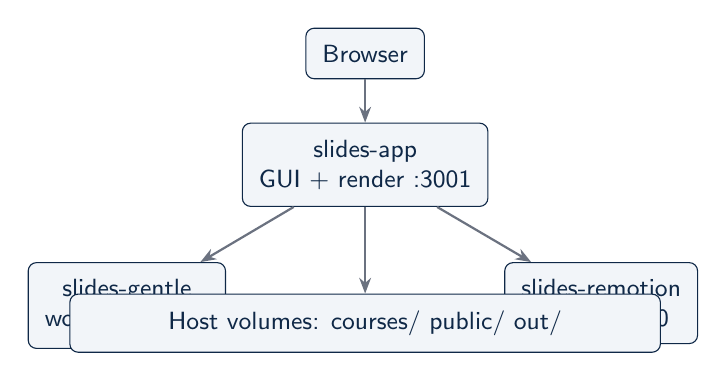
\begin{tikzpicture}[node distance=0.55cm and 0.9cm]
	\node[mnode] (user) {Browser};
	\node[mnode, below=of user] (app) {slides-app\\GUI + render :3001};
	\node[mnode, below left=0.7cm and 0.2cm of app] (gentle) {slides-gentle\\word alignment};
	\node[mnode, below right=0.7cm and 0.2cm of app] (rem) {slides-remotion\\Studio :3000};
	\node[mnode, below=1.1cm of app, minimum width=7.5cm] (vol) {Host volumes: courses/ public/ out/};
	\draw[marr] (user) -- (app);
	\draw[marr] (app) -- (gentle);
	\draw[marr] (app) -- (rem);
	\draw[marr] (app) -- (vol);
\end{tikzpicture}
\caption{System architecture. The app container serves the GUI and runs headless Remotion renders.}
\label{fig:architecture}
\end{figure}
}

\newcommand{\diagramDeployFlow}{%
\begin{figure}[htbp]
\centering
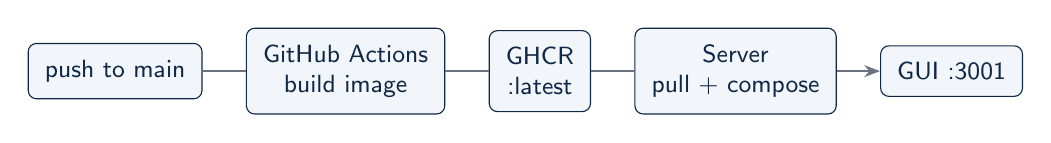
\begin{tikzpicture}[node distance=0.45cm and 0.55cm, every node/.style={mnode}]
	\node (dev) {push to main};
	\node[right=of dev] (gha) {GitHub Actions\\build image};
	\node[right=of gha] (ghcr) {GHCR\\:latest};
	\node[right=of ghcr] (host) {Server\\pull + compose};
	\node[right=of host] (gui) {GUI :3001};
	\draw[marr] (dev) -- (gha) -- (ghcr) -- (host) -- (gui);
\end{tikzpicture}
\caption{Deployment flow. Portainer or \texttt{start.sh} pulls the image; course data stays on host volumes.}
\label{fig:deploy}
\end{figure}
}

\newcommand{\diagramBootstrap}{%
\begin{figure}[htbp]
\centering
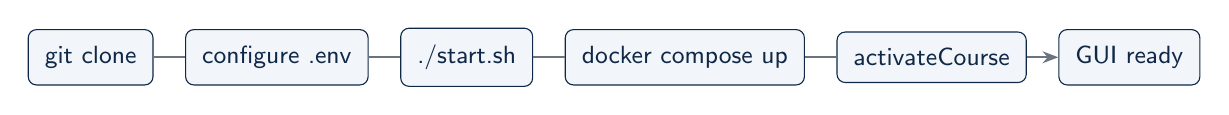
\begin{tikzpicture}[node distance=0.5cm and 0.4cm, every node/.style={mnode}]
	\node (a) {git clone};
	\node[right=of a] (b) {configure .env};
	\node[right=of b] (c) {./start.sh};
	\node[right=of c] (d) {docker compose up};
	\node[right=of d] (e) {activateCourse};
	\node[right=of e] (f) {GUI ready};
	\draw[marr] (a) -- (b) -- (c) -- (d) -- (e) -- (f);
\end{tikzpicture}
\caption{Reproduction bootstrap on a fresh server.}
\label{fig:bootstrap}
\end{figure}
}

\newcommand{\diagramWizard}{%
\begin{figure}[htbp]
\centering
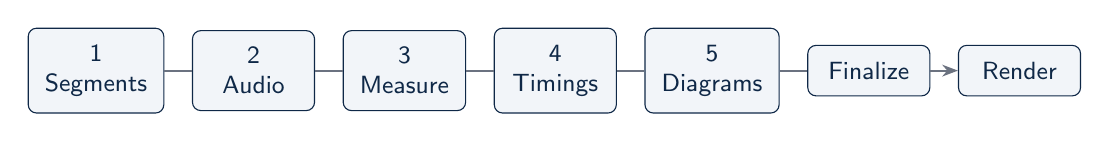
\begin{tikzpicture}[node distance=0.35cm and 0.35cm, every node/.style={mnode, minimum width=1.55cm}]
	\node (s1) {1\\Segments};
	\node[right=of s1] (s2) {2\\Audio};
	\node[right=of s2] (s3) {3\\Measure};
	\node[right=of s3] (s4) {4\\Timings};
	\node[right=of s4] (s5) {5\\Diagrams};
	\node[right=of s5] (fin) {Finalize};
	\node[right=of fin] (ren) {Render};
	\draw[marr] (s1) -- (s2) -- (s3) -- (s4) -- (s5) -- (fin) -- (ren);
\end{tikzpicture}
\caption{Processing wizard pipeline. Scene courses skip Step 5 (Mermaid) and use pre-built SVG scenes.}
\label{fig:wizard}
\end{figure}
}

\newcommand{\diagramSceneCourse}{%
\begin{figure}[htbp]
\centering
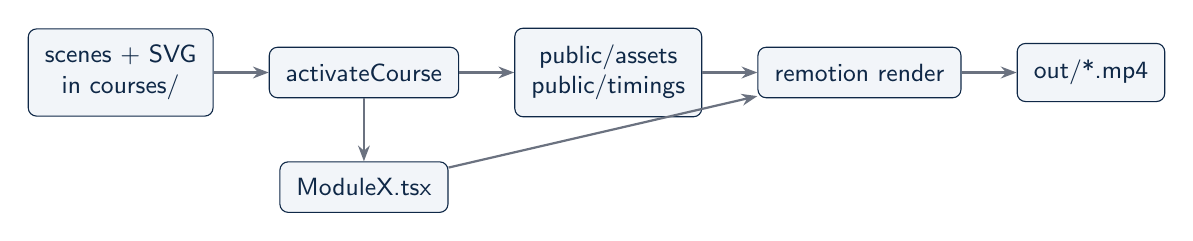
\begin{tikzpicture}[node distance=0.55cm and 0.7cm]
	\node[mnode] (scenes) {scenes + SVG\\in courses/};
	\node[mnode, right=of scenes] (act) {activateCourse};
	\node[mnode, right=of act] (pub) {public/assets\\public/timings};
	\node[mnode, below=0.8cm of act] (mod) {ModuleX.tsx};
	\node[mnode, right=of pub] (rem) {remotion render};
	\node[mnode, right=of rem] (mp4) {out/*.mp4};
	\draw[marr] (scenes) -- (act);
	\draw[marr] (act) -- (pub);
	\draw[marr] (act) -- (mod);
	\draw[marr] (pub) -- (rem);
	\draw[marr] (mod) -- (rem);
	\draw[marr] (rem) -- (mp4);
\end{tikzpicture}
\caption{Scene course path (e.g.\ agentic-ai-for-beginners). Animation uses SVG + \texttt{.animation.json}, not Mermaid.}
\label{fig:scene}
\end{figure}
}

\newcommand{\diagramBatchRender}{%
\begin{figure}[htbp]
\centering

\begin{tikzpicture}[node distance=0.5cm and 0.5cm, every node/.style={mnode}]
	\node (gui) {GUI batch render};
	\node[right=of gui] (sync) {sync assets};
	\node[right=of sync] (batch) {renderAllModules};
	\node[right=of batch] (skip) {skip existing?};
	\node[right=of skip] (out) {out/courseId/};
	\draw[marr] (gui) -- (sync) -- (batch) -- (skip) -- (out);
\end{tikzpicture}
\caption{Batch render. Skips valid MP4s by default; use force to re-render all modules.}
\label{fig:batch}
\end{figure}
}

\newcommand{\diagramGitPolicy}{%
\begin{figure}[htbp]
\centering
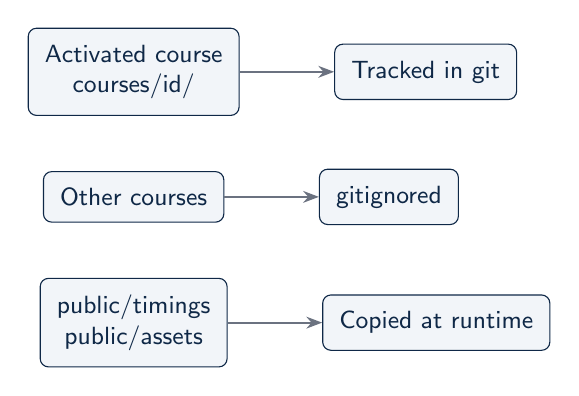
\begin{tikzpicture}[node distance=0.6cm and 1.2cm]
	\node[mnode] (active) {Activated course\\courses/id/};
	\node[mnode, right=of active] (git) {Tracked in git};
	\node[mnode, below=0.7cm of active] (arch) {Other courses};
	\node[mnode, right=of arch] (ign) {gitignored};
	\node[mnode, below=0.7cm of arch] (rt) {public/timings\\public/assets};
	\node[mnode, right=of rt] (copy) {Copied at runtime};
	\draw[marr] (active) -- (git);
	\draw[marr] (arch) -- (ign);
	\draw[marr] (rt) -- (copy);
\end{tikzpicture}
\caption{Git deploy policy: only the active course ships in the repository.}
\label{fig:gitpolicy}
\end{figure}
}

\newcommand{\diagramSoftwareLayers}{%
\begin{figure}[htbp]
\centering
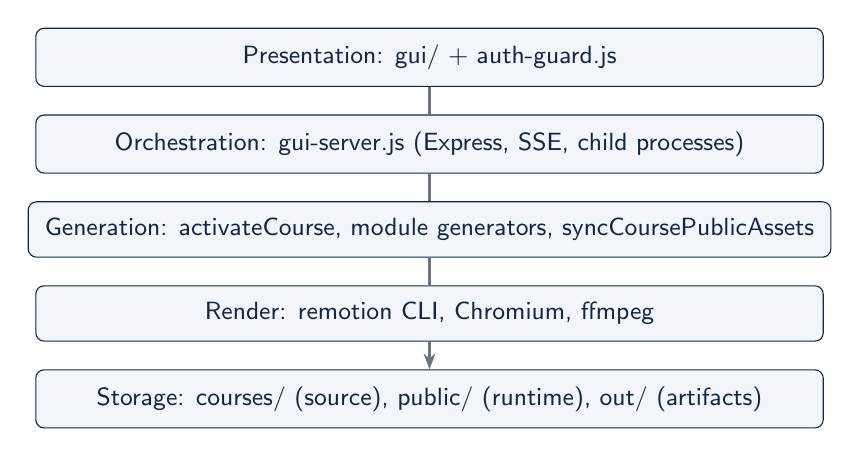
\begin{tikzpicture}[node distance=0.35cm and 0.5cm]
	\node[mnode, minimum width=10cm] (ui) {Presentation: gui/ + auth-guard.js};
	\node[mnode, minimum width=10cm, below=of ui] (orch) {Orchestration: gui-server.js (Express, SSE, child processes)};
	\node[mnode, minimum width=10cm, below=of orch] (gen) {Generation: activateCourse, module generators, syncCoursePublicAssets};
	\node[mnode, minimum width=10cm, below=of gen] (ren) {Render: remotion CLI, Chromium, ffmpeg};
	\node[mnode, minimum width=10cm, below=of ren] (store) {Storage: courses/ (source), public/ (runtime), out/ (artifacts)};
	\draw[marr] (ui) -- (orch) -- (gen) -- (ren) -- (store);
\end{tikzpicture}
\caption{Layered software architecture.}
\label{fig:layers}
\end{figure}
}

\newcommand{\diagramActivatePipeline}{%
\begin{figure}[htbp]
\centering

\begin{tikzpicture}[node distance=0.45cm and 0.4cm, every node/.style={mnode}]
	\node (a) {content.json};
	\node[right=of a] (b) {moduleContent.ts};
	\node[right=of b] (c) {public/timings};
	\node[right=of c] (d) {SVG or Mermaid};
	\node[right=of d] (e) {ModuleX.tsx};
	\node[right=of e] (f) {courses.json};
	\draw[marr] (a) -- (b) -- (c) -- (d) -- (e) -- (f);
\end{tikzpicture}
\caption{Course activation pipeline (single entry point for Remotion readiness).}
\label{fig:activate}
\end{figure}
}

\newcommand{\diagramRenderSequence}{%
\begin{figure}[htbp]
\centering
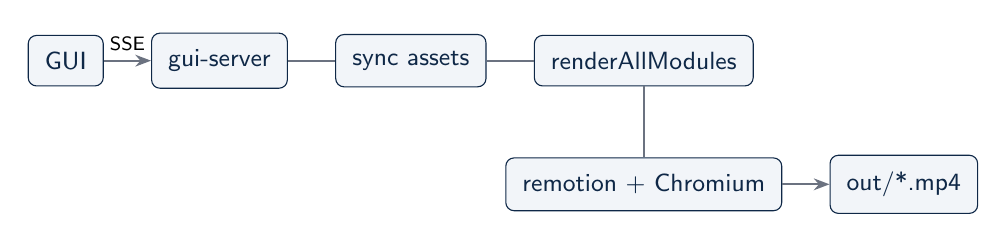
\begin{tikzpicture}[node distance=0.5cm and 0.6cm]
	\node[mnode] (ui) {GUI};
	\node[mnode, right=of ui] (api) {gui-server};
	\node[mnode, right=of api] (sync) {sync assets};
	\node[mnode, right=of sync] (batch) {renderAllModules};
	\node[mnode, below=0.9cm of batch] (rem) {remotion + Chromium};
	\node[mnode, right=of rem] (mp4) {out/*.mp4};
	\draw[marr] (ui) -- node[above, font=\scriptsize\sffamily] {SSE} (api);
	\draw[marr] (api) -- (sync) -- (batch) -- (rem) -- (mp4);
\end{tikzpicture}
\caption{Batch render control flow. Browser refresh closes SSE but does not stop the child process.}
\label{fig:renderseq}
\end{figure}
}


\hypersetup{
	colorlinks=true,
	linkcolor=rbnavy,
	urlcolor=rbred,
	citecolor=rbnavy
}

\newcommand{\rbline}{\noindent\textcolor{rbnavy}{\rule{\textwidth}{1.2pt}}\par}
\newcolumntype{L}{>{\raggedright\arraybackslash}X}
\newcommand{\tableheadrow}[1]{\sffamily\bfseries\color{rbnavy} #1}

\titleformat{\section}{\large\sffamily\bfseries\color{scinexusblue}}{}{0em}{}
\titleformat{\subsection}{\normalsize\sffamily\bfseries\color{scinexusblue}}{}{0em}{}
\titlespacing*{\section}{0pt}{1em}{0.35em}
\titlespacing*{\subsection}{0pt}{0.75em}{0.25em}

\newsavebox{\summaryboxcontent}
\newenvironment{executivesummary}{%
	\vspace{0.25em}%
	\noindent{\large\sffamily\bfseries\color{scinexusblue} Summary}\par
	\vspace{0.45em}%
	\setlength{\fboxsep}{10pt}%
	\setlength{\fboxrule}{0.8pt}%
	\begin{lrbox}{\summaryboxcontent}%
	\begin{minipage}{\dimexpr\textwidth-2\fboxsep-2\fboxrule\relax}%
	\setlength{\parskip}{0.5em}%
}{%
	\end{minipage}%
	\end{lrbox}%
	\noindent\fcolorbox{summaryborder}{summarybg}{\usebox{\summaryboxcontent}}%
	\vspace{0.75em}%
}

\setlength{\parskip}{0.5em}
\renewcommand{\arraystretch}{1.12}

\newlength{\coverheadheight}
\newlength{\coverheadpadding}
\newsavebox{\coverlogobox}
\newsavebox{\coverheaderbox}
\newcommand{\setcoverlogo}{%
	\setlength{\coverheadpadding}{14pt}%
	\savebox{\coverlogobox}{%
		
\includegraphics[width=0.55\textwidth,keepaspectratio]{logo.png}%
	}%
	\savebox{\coverheaderbox}{%
		\rule{0pt}{\coverheadpadding}%
		\usebox{\coverlogobox}%
	}%
	\setlength{\coverheadheight}{\dimexpr\ht\coverheaderbox+\dp\coverheaderbox\relax}%
}

\fancypagestyle{coverpage}{%
	\fancyhf{}%
	\fancyhead[L]{\usebox{\coverheaderbox}}%
	\renewcommand{\headrulewidth}{0pt}%
	\cfoot{}%
}

\newcommand{\systemcover}{%
	\setcoverlogo
	\newgeometry{top=1.45in, headheight=\coverheadheight, headsep=5pt}%
	\thispagestyle{coverpage}%
	\rbline\vspace{-0.4em}%
	\vspace{0.85em}%
	{\large\sffamily\bfseries\color{rbnavy} System \color{rbred}Guide}\\[1.25em]%
	\noindent\parbox{\textwidth}{%
		{\fontsize{19}{35}\selectfont\sffamily\bfseries\color{rbnavy} AI Video Animation Platform}%
	}\\[0.65em]%
	\noindent{\large\sffamily\color{rbgray} Engineering, architecture, and operations}%
	\rbline
	\vfill
	{\small\sffamily
	Repository: \href{https://github.com/f2ka07/AI-video-animation}{f2ka07/AI-video-animation}}%
	\par\vspace{0.5em}%
	\restoregeometry
}

\fancypagestyle{body}{%
	\fancyhf{}%
	\renewcommand{\headrulewidth}{0pt}%
	\cfoot{\small\sffamily\thepage}%
}

\begin{document}

\systemcover
\pagestyle{body}

\begin{executivesummary}

This document explains \textbf{how the AI Video Animation platform is engineered}---layers, data models, generation pipelines, Remotion integration, and deploy policy---and how to \textbf{operate} it on EC2, RunPod, or Portainer.

The stack is a Node.js monorepo: Express orchestrates long-running media jobs; Remotion renders React compositions to MP4 via headless Chromium; course content lives on host volumes while the Docker image carries application code only.

\end{executivesummary}

\part{System Engineering}

\section{Design Principles}

The codebase follows a small set of architectural rules that explain most file boundaries:

\begin{table}[htbp]
	\centering
	\footnotesize
	\caption{Engineering principles}
	\begin{tabularx}{\textwidth}{@{}L L@{}}
		\toprule
		\tableheadrow{Principle} & \tableheadrow{Rationale} \\
		\midrule
		Source vs runtime split & \texttt{courses/} holds authoritative content; \texttt{public/} is what Remotion reads at render time \\
		Code generation over hand-editing & \texttt{moduleContent.ts} and \texttt{ModuleX.tsx} are regenerated by scripts to avoid drift \\
		Two visual pipelines & Generic slides (Mermaid + auto animation) vs scene courses (React scenes + SVG) share one GUI \\
		Child-process renders & \texttt{gui-server.js} spawns \texttt{remotion render}; no in-process Chromium in Express \\
		Single active course in git & Deploy policy keeps one \texttt{courses/<id>/} tracked; reduces image size and confusion \\
		Volume-first production & MP4s, timings, and copied assets survive container replacement \\
		\bottomrule
	\end{tabularx}
\end{table}

\section{Layered Architecture}

\diagramSoftwareLayers

\begin{description}
	\item[Presentation] Static HTML/JS in \texttt{gui/}. The processing wizard calls REST endpoints and consumes Server-Sent Events (SSE) during renders. \texttt{auth-guard.js} attaches \texttt{X-Gui-Token} to API calls after login.
	\item[Orchestration] \texttt{gui-server.js} --- single Express app on port 3001. Routes planning, audio, timings, activation, and render APIs. Spawns \texttt{tsx} / \texttt{npx remotion} child processes with streamed stdout for progress.
	\item[Generation] TypeScript scripts under \texttt{scripts/} transform \texttt{content.json} into Remotion-ready artifacts (\texttt{moduleContent.ts}, \texttt{ModuleX.tsx}, animation specs, public copies).
	\item[Render] Remotion CLI bundles \texttt{src/index.tsx}, drives Chromium frame capture, encodes MP4. Concurrency capped by \texttt{renderConcurrency.js} (cgroup-aware).
	\item[Storage] Host-mounted directories. The Docker image excludes generated \texttt{public/assets}, \texttt{public/timings}, and \texttt{out/} (see \texttt{.dockerignore}).
\end{description}

\section{Docker Image vs Host State}

The Dockerfile builds one image (\texttt{node:20-slim} + Chromium) used by both \texttt{slides-app} and optional \texttt{slides-remotion}. Application code is copied at build time; \textbf{course and render data are not}.

\begin{table}[htbp]
	\centering
	\footnotesize
	\caption{What lives where}
	\begin{tabularx}{\textwidth}{@{}l l L@{}}
		\toprule
		\tableheadrow{Location} & \tableheadrow{In image?} & \tableheadrow{Contents} \\
		\midrule
		\texttt{/app/src}, \texttt{gui-server.js} & Yes & Remotion entry, generated modules \\
		\texttt{courses/} & Partial & Active course tracked in git; mounted at runtime \\
		\texttt{public/audio/<course>} & Partial & Whitelisted WAVs for active course \\
		\texttt{public/assets/} & No & SVG + animation JSON copied before render \\
		\texttt{public/timings/} & No & Word timing JSON copied from \texttt{courses/} \\
		\texttt{out/} & No & Rendered MP4 outputs \\
		\bottomrule
	\end{tabularx}
\end{table}

Compose mounts \texttt{./src}, \texttt{./gui}, \texttt{./scripts}, and \texttt{gui-server.js} as volumes in development so code changes apply without rebuild. Production typically uses the GHCR image plus host volumes for data.

\section{Course Visual Modes}

Mode detection is centralized in \texttt{scripts/courseVisualMode.ts}. A course is a \textbf{scene course} if \texttt{courses/<id>/course/remotion/scenes} exists or \texttt{courses.json} marks \texttt{visualMode: "scenes"}.

\begin{table}[htbp]
	\centering
	\footnotesize
	\caption{Generic vs scene engineering}
	\begin{tabularx}{\textwidth}{@{}l L L@{}}
		\toprule
		\tableheadrow{Aspect} & \tableheadrow{Generic slides} & \tableheadrow{Scene course} \\
		\midrule
		Remotion modules & \texttt{generateModulesFromContent.ts} & \texttt{generateModulesFromScenes.ts} \\
		Slides & \texttt{GenericModule} + slide types & Per-scene React components \\
		Diagrams & Mermaid $\rightarrow$ SVG pipeline & Hand-authored SVG in repo \\
		Animation & \texttt{generateAnimationSpecs.ts} (auto) & Hand-tuned \texttt{.animation.json} \\
		Wizard Step 5 & Mermaid classify/generate & Disabled \\
		Intro/Recap & From slide scripts & Dedicated scene components \\
		\bottomrule
	\end{tabularx}
\end{table}

Scene courses strip Mermaid fields from content plans on activate so generic diagram tooling never overwrites SVG assets.

\section{Content and Timing Model}

\subsection{Authoritative sources}

\begin{itemize}
	\item \texttt{courses/<id>/content.json} --- modules, slides, scripts, bullet points (planning output or hand-edited).
	\item \texttt{courses/<id>/timings/moduleN.json} --- per-slide word arrays \texttt{\{text, start, end\}} used for bullet highlights and diagram phases.
	\item \texttt{courses/<id>/course/remotion/scenes/} --- scene components (scene courses only).
	\item \texttt{courses/<id>/course/diagrams/svg/} --- SVG sources and animation specs (scene courses).
\end{itemize}

\subsection{Generated Remotion inputs}

\texttt{activateCourse.ts} writes \texttt{src/videos/moduleContent.ts} --- the TypeScript module list Remotion and the GUI treat as source of truth (header comment includes \texttt{Course ID}). It also copies timings into \texttt{public/timings/} because Remotion's \texttt{staticFile("timings/...")} reads from \texttt{public/}, not \texttt{courses/}.

\subsection{Composition structure}

\texttt{src/Root.tsx} registers one Remotion composition per module (\texttt{module-1}, \texttt{module-2}, \ldots). Each \texttt{src/videos/ModuleN.tsx} is a \texttt{Series} of scenes with durations derived from \texttt{audioDuration.ts} and cue points from timings JSON.

\section{Course Activation Pipeline}

Activation is the \textbf{commit point} that makes a course renderable. Invoked by \texttt{start.sh}, the GUI finalize step, or \texttt{POST /api/courses/:id/activate}.

\diagramActivatePipeline

\begin{enumerate}
	\item Load \texttt{content.json}; generate \texttt{moduleContent.ts}.
	\item Copy \texttt{courses/<id>/timings/*.json} $\rightarrow$ \texttt{public/timings/}.
	\item Scene course: \texttt{copySvgsToPublic.ts} $\rightarrow$ \texttt{public/assets/<id>/}. Generic: \texttt{generateAnimationSpecs.ts} first.
	\item Regenerate \texttt{ModuleX.tsx} via scene or content generator.
	\item Update \texttt{courses.json} active/archived flags; run \texttt{courseDeployPolicy.js} to sync \texttt{.gitignore} markers.
\end{enumerate}

\texttt{syncCoursePublicAssets.js} (called before each render) repeats the timings + SVG copy so headless render never sees stale or empty \texttt{public/assets}.

\section{Remotion Module Generation}

\subsection{Scene path (\texttt{generateModulesFromScenes.ts})}

Scans \texttt{course/remotion/scenes/moduleNN/} for components (\texttt{Module01Intro}, \texttt{Module01Diagram1}, etc.). Builds a \texttt{Series} with:

\begin{itemize}
	\item Duration from \texttt{audioDuration.ts} keys (\texttt{courseId-module-N-scene}).
	\item \texttt{cuePoints} --- frame indices from word timings for diagram scenes.
	\item Imports resolved to course-local scene files, not generic slide components.
\end{itemize}

\subsection{Generic path (\texttt{generateModulesFromContent.ts})}

Maps slide types (\texttt{content-two-card}, \texttt{code}, \texttt{mermaid}, etc.) to React slide components under \texttt{src/components/}. Bullet visibility uses word timings via shared slide utilities.

\section{Diagram Animation Engine}

Scene diagrams use \texttt{BaseDiagramScene.tsx} in the course's \texttt{remotion/shared/} folder.

\subsection{Asset loading}

At runtime in Chromium, the scene calls \texttt{fetch(staticFile(svgPath))} where \texttt{svgPath} is relative to \texttt{public/} (e.g.\ \texttt{assets/<course>/module01/foo.svg}). \texttt{delayRender}/\texttt{continueRender} block the frame pipeline until SVG and optional \texttt{.animation.json} load --- required for headless export.

\subsection{Phase resolution}

Each \texttt{.animation.json} defines \texttt{phases[]} with \texttt{show}, \texttt{dim}, and \texttt{highlight} group IDs matching \texttt{<g id="...">} in the SVG. When word timings and \texttt{slideName} are available, \texttt{BaseDiagramScene} prefers \textbf{word-driven phase boundaries} over static \texttt{start}/\texttt{end} seconds in the spec --- keeping diagram reveals aligned with narration.

\subsection{Why not AI-only SVG}

AI-generated SVG without structured group IDs and a matching animation spec renders as a static image. The Agentic course quality depends on the \textbf{pair} (SVG structure + phased JSON + timings), not the SVG file alone.

\section{Render Pipeline}

\diagramRenderSequence

\subsection{Single module}

\texttt{POST /api/render-video} runs \texttt{npx remotion render src/index.tsx module-N out/...} with SSE progress parsed from Remotion stdout (bundling, \texttt{Rendered X/Y}, encoding).

\subsection{Batch}

\texttt{POST /api/render-course} spawns \texttt{renderAllModules.ts}, which loops modules sequentially. Each iteration uses async \texttt{spawn} (not \texttt{spawnSync}) so progress streams live. \texttt{--skip-existing} skips MP4s over 100\,KB unless \texttt{--force}.

\subsection{Concurrency}

\texttt{scripts/lib/renderConcurrency.js} reads cgroup CPU limits when present (Docker/EC2), subtracts \texttt{REMOTION\_CPU\_RESERVE}, and caps \texttt{--concurrency}. Prevents Remotion from requesting more Chromium tabs than vCPUs allow.

\section{GUI Server API Surface}

The API is grouped by responsibility (all under \texttt{/api/}, auth required except login/status):

\begin{table}[htbp]
	\centering
	\footnotesize
	\caption{API groups}
	\begin{tabularx}{\textwidth}{@{}l L@{}}
		\toprule
		\tableheadrow{Group} & \tableheadrow{Examples} \\
		\midrule
		Course lifecycle & \texttt{/plan-course}, \texttt{/courses}, \texttt{/courses/:id/activate} \\
		Module editing & \texttt{/modules}, \texttt{/modules/:n/improve}, \texttt{/slide-splits} \\
		Media pipeline & \texttt{/generate-audio}, \texttt{/measure-audio}, \texttt{/align-diagram-phases} \\
		Remotion & \texttt{/generate-modules}, \texttt{/regenerate-modules}, \texttt{/check-scene-components} \\
		Render & \texttt{/render-video}, \texttt{/render-course}, \texttt{/render-runpod} \\
		Voice & \texttt{/voice-settings}, \texttt{/voices/test} \\
		System & \texttt{/health}, \texttt{/system-info}, \texttt{/auth/login} \\
		\bottomrule
	\end{tabularx}
\end{table}

Long operations use SSE (\texttt{text/event-stream}) or subprocess stdout parsing --- not WebSockets.

\section{Git Deploy Policy}

\texttt{scripts/lib/courseDeployPolicy.js} maintains marked sections in \texttt{.gitignore}:

\begin{itemize}
	\item \texttt{courses/*} ignored except \texttt{!courses/<activeId>/}
	\item \texttt{public/audio/*} ignored except whitelisted course folder
	\item \texttt{public/timings/} always ignored (runtime copy)
\end{itemize}

On activate, archived courses are removed from the git index (\texttt{git rm --cached}). CI in \texttt{.github/workflows/deploy.yml} verifies only one course is tracked. Manifest written to \texttt{workspace/deploy-manifest.json}.

\section{Security Model}

When \texttt{GUI\_AUTH\_PASSWORD} is set:

\begin{itemize}
	\item \texttt{POST /api/auth/login} compares credentials; returns \texttt{GUI\_SESSION\_SECRET} or a hash derived from the password as \texttt{token}.
	\item Client stores token in \texttt{sessionStorage}; \texttt{auth-guard.js} sends \texttt{X-Gui-Token} on API requests.
	\item Middleware protects \textbf{API routes only} --- static HTML loads in the browser; unauthenticated users cannot call pipeline APIs.
	\item Changing \texttt{.env} requires \texttt{docker compose up -d --force-recreate app} --- restart alone does not reload env.
\end{itemize}

Secrets (\texttt{OPENAI\_API\_KEY}, voice keys) never belong in the image; they are injected via Compose environment from host \texttt{.env}.

\section{Extension Points}

\begin{table}[htbp]
	\centering
	\footnotesize
	\caption{Where to extend the system}
	\begin{tabularx}{\textwidth}{@{}l L@{}}
		\toprule
		\tableheadrow{Goal} & \tableheadrow{Touch points} \\
		\midrule
		New scene course & \texttt{courses/<id>/course/remotion/scenes/}, SVG + animation JSON, \texttt{courses.json} mapping \\
		New slide type (generic) & \texttt{src/components/}, generator in \texttt{generateModulesFromContent.ts} \\
		New TTS provider & \texttt{gui-server.js} voice routes, \texttt{workspace/config} voice settings \\
		Remote render & \texttt{renderOnRunPod.ts}, \texttt{POST /api/render-runpod} \\
		CI/deploy & \texttt{.github/workflows/deploy.yml}, \texttt{docker-compose.prod.yml} \\
		\bottomrule
	\end{tabularx}
\end{table}

\part{Operations Guide}

\section{Purpose}

The platform turns structured course content into narrated slide videos. Two course modes exist:

\begin{itemize}
	\item \textbf{Generic slides} --- bullet/code slides with optional Mermaid diagrams; animation specs generated from word timings.
	\item \textbf{Scene courses} --- custom Remotion scenes with hand-tuned SVG diagrams and \texttt{.animation.json} phase files (e.g.\ \texttt{agentic-ai-for-beginners}).
\end{itemize}

The same Docker stack serves both: GUI on port \textbf{3001}, Gentle for alignment, optional Remotion Studio on \textbf{3000}.

\section{System Architecture}

\diagramSystemArchitecture

\begin{table}[htbp]
	\centering
	\footnotesize
	\caption{Docker services}
	\label{tab:services}
	\begin{tabularx}{\textwidth}{@{}l l L@{}}
		\toprule
		\tableheadrow{Service} & \tableheadrow{Port} & \tableheadrow{Role} \\
		\midrule
		slides-app & 3001 & Web GUI, pipeline APIs, headless Remotion render \\
		slides-gentle & internal & Word-level timing extraction (wizard Step 4) \\
		slides-remotion & 3000 (localhost) & Remotion Studio preview (optional profile) \\
		\bottomrule
	\end{tabularx}
\end{table}

Host directories mounted into the app container:

\begin{itemize}
	\item \texttt{courses/} --- course scripts, scenes, SVG sources, timings in git
	\item \texttt{public/} --- runtime audio, copied assets, timings for Remotion
	\item \texttt{out/} --- rendered MP4 files
	\item \texttt{workspace/} --- local config and logs
\end{itemize}

\section{Deployment Flow}

\diagramDeployFlow

Push to \texttt{main} triggers GitHub Actions to build and push \texttt{ghcr.io/f2ka07/ai-video-animation:latest}. The server pulls the image and runs \texttt{docker-compose.prod.yml} or \texttt{start.sh}. Course content on host volumes is \textbf{not} overwritten by image updates.

\section{Reproduce on a Fresh Server}

\diagramBootstrap

\subsection{Prerequisites}

\begin{itemize}
	\item Ubuntu 22.04+ (or similar Linux), 16+ GB disk, 8+ vCPU recommended for batch render
	\item Security group / firewall: TCP \textbf{3001} open for GUI (restrict by IP in production)
	\item GitHub access to clone the repository
\end{itemize}

\subsection{Steps}

\begin{enumerate}
	\item Clone: \texttt{git clone git@github.com:f2ka07/AI-video-animation.git}
	\item Copy \texttt{.env.example} to \texttt{.env}; set \texttt{GUI\_AUTH\_PASSWORD}, \texttt{OPENAI\_API\_KEY}, optional \texttt{SLIDES\_IMAGE}
	\item First boot: \texttt{INSTALL\_DOCKER=1 ./start.sh}
	\item Later restarts: \texttt{./start.sh}
	\item Open \texttt{http://<server-ip>:3001}, sign in, open \textbf{Video Processing} wizard
\end{enumerate}

RunPod: \texttt{USE\_HOST\_NETWORK=1 ./start.sh}

\section{Processing Wizard}

\diagramWizard

\begin{table}[htbp]
	\centering
	\footnotesize
	\caption{Wizard steps}
	\begin{tabularx}{\textwidth}{@{}c L@{}}
		\toprule
		\tableheadrow{Step} & \tableheadrow{Action} \\
		\midrule
		1 & Edit / generate segment scripts (OpenAI planning) \\
		2 & Generate TTS audio per module \\
		3 & Measure audio duration per slide \\
		4 & Extract word timings (Gentle or Whisper) \\
		5 & Diagram pipeline (Mermaid courses only) \\
		Finalize & Activate course, rebuild Remotion modules \\
		Render & Single module or batch overnight (Local target on server) \\
		\bottomrule
	\end{tabularx}
\end{table}

Scene courses: Step 5 is disabled; diagrams live under \texttt{courses/<id>/course/diagrams/svg/}. Use \textbf{Finalize Video} or \texttt{activateCourse.ts} after Step 4.

\section{Scene Course Data Flow}

\diagramSceneCourse

Remotion resolves diagram paths via \texttt{staticFile("assets/<course>/module01/...")} --- relative to \texttt{public/}, not absolute URLs. Before render, \texttt{syncCoursePublicAssets} copies SVGs and timings from \texttt{courses/} into \texttt{public/}.

Each scene diagram needs:
\begin{itemize}
	\item SVG with \texttt{<g id="...">} groups for animated parts
	\item Matching \texttt{.animation.json} with \texttt{phases} (show / dim / highlight)
	\item Word timings in \texttt{public/timings/moduleN.json} for narration sync
\end{itemize}

\section{Batch Render}

\diagramBatchRender

In the GUI: set \textbf{Render on: Local}, optionally check \textbf{Re-render modules that already have MP4}. Default skips existing outputs. Progress shows overall course percent plus per-module bars.

CLI equivalent:

\begin{itemize}
	\item \texttt{npm run render:course -- --course=agentic-ai-for-beginners}
	\item \texttt{--force} to re-render all; omit to skip existing MP4s
\end{itemize}

Refreshing the browser does \textbf{not} stop a running render; monitor with \texttt{docker logs -f slides-app}.

\section{Git Deploy Policy}

\diagramGitPolicy

Only the \textbf{activated} course is tracked in git under \texttt{courses/<id>/}. Runtime folders \texttt{public/timings/} and \texttt{public/assets/} are copied at activate/render time and are not required in the Docker image.

\section{Environment Variables}

\begin{table}[htbp]
	\centering
	\footnotesize
	\caption{Key \texttt{.env} variables}
	\begin{tabularx}{\textwidth}{@{}l L@{}}
		\toprule
		\tableheadrow{Variable} & \tableheadrow{Purpose} \\
		\midrule
		SLIDES\_COURSE\_ID & Course activated by \texttt{start.sh} \\
		SLIDES\_IMAGE & GHCR image tag for production compose \\
		GUI\_AUTH\_USERNAME / GUI\_AUTH\_PASSWORD & GUI login (required on cloud) \\
		OPENAI\_API\_KEY & Course planning and OpenAI TTS \\
		REMOTION\_CONCURRENCY & Cap render threads (e.g.\ 14 on 16 vCPU) \\
		REMOTION\_CPU\_RESERVE & Cores left for OS/GUI (default 1) \\
		GENTLE\_URL / REMOTION\_URL & Internal Docker service URLs \\
		\bottomrule
	\end{tabularx}
\end{table}

After changing \texttt{.env}, recreate the app container: \texttt{docker compose up -d --force-recreate app}.

\section{Mermaid Diagram Sources}

Editable Mermaid sources live in \texttt{ProductionStacks/diagrams/*.mmd}. To regenerate figures:

\begin{enumerate}
	\item Open any \texttt{.mmd} file in \href{https://mermaid.live}{mermaid.live}, or
	\item Run \texttt{npx @mermaid-js/mermaid-cli -i diagrams/NAME.mmd -o figures/NAME.png}
\end{enumerate}

Example architecture source:

\begin{mermaidsource}
flowchart TB
  USER[Browser] --> APP[slides-app :3001]
  APP --> GENTLE[gentle]
  APP --> PUBLIC[public/ assets timings]
  APP --> OUT[out/ MP4s]
\end{mermaidsource}

\section{Common Issues}

\begin{table}[htbp]
	\centering
	\footnotesize
	\begin{tabularx}{\textwidth}{@{}L L@{}}
		\toprule
		\tableheadrow{Symptom} & \tableheadrow{Fix} \\
		\midrule
		Blank / missing diagrams in MP4 & Run \texttt{activateCourse.ts}; verify \texttt{public/assets/<course>/} \\
		Login succeeds but returns to login page & Pull latest GUI auth fix; restart app \\
		Batch render transform error & Pull latest \texttt{renderAllModules.ts}; restart app \\
		Progress stuck at low \% & Normal while a long module renders; check \texttt{docker logs} \\
		\bottomrule
	\end{tabularx}
\end{table}

\section{Repository Map}

\begin{table}[htbp]
	\centering
	\footnotesize
	\begin{tabularx}{\textwidth}{@{}l L@{}}
		\toprule
		\tableheadrow{Path} & \tableheadrow{Role} \\
		\midrule
		start.sh & Server bootstrap and course activation \\
		docker-compose.yml / .prod.yml & Service definitions \\
		gui-server.js & API, auth, render orchestration \\
		gui/ & Web UI and processing wizard \\
		scripts/activateCourse.ts & Activate course for Remotion \\
		scripts/renderAllModules.ts & Batch MP4 render \\
		courses/<id>/ & Course content and scenes \\
		src/videos/ & Generated ModuleX.tsx compositions \\
		\bottomrule
	\end{tabularx}
\end{table}

\vspace{1em}
\noindent{\small\sffamily\itshape
Part I documents system engineering; Part II documents deployment and daily operation. Update \texttt{diagrams/*.mmd} when architecture changes, then refresh TikZ in \texttt{diagrams/tikz-figures.tex}.}

\end{document}
